\documentclass[12pt]{article}

% --- Paquetes Requeridos para Estilo APA y Formato ---
\usepackage[spanish,es-tabla]{babel} % Configuración para idioma español y etiquetas de tablas
\usepackage{geometry}
\geometry{
    a4paper,
    margin=1in % Margen de 1 pulgada (2.54 cm) requerido por APA
}

\usepackage{setspace}
\doublespacing % Espaciado doble requerido por APA
\usepackage{fontspec} % Requerido en LuaLaTeX para fuentes tipográficas
\setmainfont{Times New Roman} % Configura Times New Roman de forma nativa para LuaLaTeX (corrige negritas)
\usepackage{indentfirst} % Indentación en el primer párrafo de cada sección
\usepackage{titlesec}
\usepackage{graphicx}
\usepackage{booktabs} % Para tablas limpias estilo APA (sin líneas verticales)
\usepackage{caption}
\usepackage{float} % Para posicionamiento preciso de tablas e imágenes (H)
\usepackage{hyperref}
\usepackage{xurl}
\usepackage{fancyhdr}

% Configuración de ruta de imágenes para buscar en la carpeta del tercer entregable
\graphicspath{{../3er_entregable/}}

% --- Configuración de Encabezado y Pie de Página (APA 7 Estudiantes) ---
\pagestyle{fancy}
\fancyhf{}
\setlength{\headheight}{15pt} % Aumenta la altura del encabezado para evitar advertencias de fancyhdr
\addtolength{\topmargin}{-3pt} % Compensa el cambio de altura del encabezado
\rhead{\thepage} % Número de página en la esquina superior derecha
\lhead{}
\renewcommand{\headrulewidth}{0pt} % Elimina la línea horizontal del encabezado

% --- Configuración de Títulos con Numeración Románica Dinámica ---
\renewcommand{\thesection}{\Roman{section}}
\titleformat{\section}{\normalfont\normalsize\bfseries\centering}{\thesection.}{0.5em}{}
\titleformat{\subsection}{\normalfont\normalsize\bfseries}{}{0pt}{}
\titleformat{\subsubsection}{\normalfont\normalsize\bfseries\itshape}{}{0pt}{}

% --- Ajuste del Ancho de Numeración en el Índice (TOC) ---
\usepackage[titles]{tocloft}
\setlength{\cftsecnumwidth}{3.2em} % Aumenta el espacio para que números romanos como VII y VIII no se choquen con el título
\setlength{\cftsubsecnumwidth}{3.8em} % Aumenta el espacio para numeración heredada como VIII.1
\setlength{\cftsubsubsecnumwidth}{4.5em}

% Ajustes de sangría de párrafos (0.5 pulgadas)
\setlength{\parindent}{0.5in}
\setlength{\parskip}{0pt}

% --- Formato APA para Leyendas de Tablas y Figuras ---
\captionsetup[table]{
    labelfont=bf,
    textfont=it,
    labelsep=newline,
    justification=justified,
    singlelinecheck=false,
    skip=10pt
}
\captionsetup[figure]{
    labelfont=bf,
    textfont=it,
    labelsep=newline,
    justification=justified,
    singlelinecheck=false,
    skip=10pt
}

\begin{document}

% ==========================================
% I. CARÁTULA
% ==========================================
\begin{titlepage}
    \centering
    \setstretch{1.1}
    
    {\fontsize{14pt}{16pt}\selectfont\bfseries UNIVERSIDAD NACIONAL AGRARIA DE LA SELVA} \\
    \vspace{0.2cm}
    {\fontsize{12pt}{14pt}\selectfont\bfseries FACULTAD DE INGENIERÍA EN INFORMÁTICA Y SISTEMAS} \\
    \vspace{0.2cm}
    {\fontsize{11pt}{13pt}\selectfont\bfseries ESCUELA PROFESIONAL DE INGENIERÍA EN INFORMÁTICA Y SISTEMAS} \\
    
    \vspace{1.2cm}
    % Logos institucionales
    \begin{minipage}{0.8\textwidth}
        \centering
        
\includegraphics[width=3.2cm]{unas.png}  
        \hspace{1.2cm}  
        
\includegraphics[width=3.2cm]{fiis_unas.jpg}
        \vspace{0.5cm}
    \end{minipage}
    
    \vspace{1.2cm}
    \rule{\textwidth}{1.6pt} \\ [0.4cm]
    {\fontsize{13pt}{15pt}\selectfont\bfseries INFORME FINAL DEL PROYECTO DE INNOVACIÓN Y TECNOLOGÍA} \\ [0.4cm]
    {\fontsize{15pt}{17pt}\selectfont\bfseries ``SISTEMA DE GESTIÓN FINANCIERA CON INTELIGENCIA ARTIFICIAL - FINANCIA!''} \\ [0.4cm]
    \rule{\textwidth}{0.4pt} \\
    
    \vspace{2.0cm}
    \begin{minipage}[t]{0.48\textwidth}
        \flushleft
        \fontsize{11pt}{13pt}\selectfont
        \textbf{Presentado por:} \\
        \vspace{0.2cm}
        \hspace{0.2cm} Esquivel Mori, Fabrizzio Fabiano \\
        \hspace{0.2cm} Alipázaga Bazán, Diogo Aarón \\
        \hspace{0.2cm} Miranda Murrieta, Sergio Wilson \\
        \hspace{0.2cm} Ildefonso Sotelo, Andrew Roy
    \end{minipage}
    \hfill
    \begin{minipage}[t]{0.48\textwidth}
        \flushleft
        \fontsize{11pt}{13pt}\selectfont
        \textbf{Curso:} \\
        \hspace{0.2cm} Innovación e Emprendimiento \\
        \vspace{0.3cm}
        \textbf{Docente:} \\
        \hspace{0.2cm} Michael Mariño Gamboa \\
        \vspace{0.3cm}
        \textbf{Fecha:} \\
        \hspace{0.2cm} 19 de julio de 2026
    \end{minipage}
    
    \vfill
    {\fontsize{11pt}{13pt}\selectfont\bfseries TINGO MARÍA – PERÚ} \\
    {\fontsize{10pt}{12pt}\selectfont 2026}
    
\end{titlepage}

\newpage

% ==========================================
% ÍNDICE GENERAL
% ==========================================
\renewcommand{\contentsname}{ÍNDICE}
\tableofcontents
\newpage

% ==========================================
% INTRODUCCIÓN
% ==========================================
\section{INTRODUCCIÓN}
En el contexto socioeconómico actual, la gestión efectiva de las finanzas personales se ha convertido en una competencia esencial para garantizar la estabilidad económica individual. Sin embargo, una gran parte de la población, en especial los estudiantes universitarios y jóvenes profesionales, experimenta serias dificultades para llevar un control riguroso de sus ingresos y egresos diarios. La principal causa de este fenómeno radica en la alta fricción cognitiva asociada a los métodos de registro tradicionales; la necesidad de anotar manualmente cada transacción (montos, categorías, establecimientos y fechas) en libretas o aplicaciones convencionales genera pereza y frustración, derivando inevitablemente en el abandono del control financiero.

Para dar respuesta a esta problemática dentro de la comunidad de la Universidad Nacional Agraria de la Selva (UNAS), se concibió y desarrolló \textbf{FinancIA!}, un asistente inteligente de gestión financiera personal. A diferencia de las aplicaciones tradicionales, FinancIA! aprovecha las capacidades de la Inteligencia Artificial generativa mediante el modelo Google Gemini para procesar el lenguaje natural. Esto permite que los usuarios registren sus movimientos cotidianos a través de comandos de texto libre o dictado por voz, eliminando los extensos formularios de entrada y reduciendo la fricción a su mínima expresión.

El presente informe final documenta de manera detallada todo el proceso de innovación, diseño e implementación del sistema. El documento se organiza de la siguiente manera:
\begin{itemize}
    \item La primera sección expone el diagnóstico del problema en el entorno de la UNAS, su priorización frente a otras problemáticas y la caracterización de los principales grupos afectados.
    \item La segunda sección describe el Producto Mínimo Viable (MVP) desarrollado, delimitando sus objetivos y alcance.
    \item La tercera sección detalla el diseño de interfaz de usuario (UI/UX) y el flujo de actividades operativo del software.
    \item La cuarta sección aborda la arquitectura técnica del sistema, incluyendo el modelo de datos relacional en SQLite y la inyección dinámica de contexto en la IA.
    \item La quinta sección proporciona el manual de instalación y ejecución en entornos de desarrollo y producción.
    \item Las secciones sexta, séptima y octava documentan la metodología de validación del MVP con los \textit{early adopters}, los resultados de satisfacción cuantitativos, la retroalimentación cualitativa obtenida y las mejoras propuestas.
    \item Finalmente, se presentan las conclusiones transversales del proyecto y las directrices para el trabajo futuro.
\end{itemize}

\newpage

% ==========================================
% DETECCIÓN Y ANÁLISIS DEL PROBLEMA
% ==========================================
\section{DETECCIÓN Y ANÁLISIS DEL PROBLEMA}

\subsection{Detección del Problema en la UNAS (Paso 1: Observar)}
El proceso de innovación comenzó con una fase de observación dentro de los diferentes entornos de la Universidad Nacional Agraria de la Selva (UNAS), incluyendo aulas, oficinas académicas, laboratorios, facultades y la cafetería. En esta etapa se identificó una lista de 10 problemas críticos que afectan de manera cotidiana a estudiantes, docentes y personal administrativo. La Tabla \ref{tab:problemas_detectados} resume los problemas detectados, su localización física y el grupo de interés impactado durante el diagnóstico inicial de Mayo de 2026.

\begin{table}[H]
\centering
\singlespacing
\caption{Lista de Problemas Detectados en el Entorno Universitario (UNAS)}
\label{tab:problemas_detectados}
\begin{tabular}{cp{5.5cm}p{3.5cm}p{5.5cm}}
\toprule
\textbf{N°} & \textbf{Problema Identificado} & \textbf{Lugar de Ocurrencia} & \textbf{A quién afecta} \\
\midrule
1 & Víctimas de extorsión guardan silencio & Oficina académica, Facultad, Cafetería & Estudiantes, Docentes y Personal administrativo \\
2 & Pérdida del rastro de los gastos & Oficina académica & Personal administrativo, Estudiantes y Docentes \\
3 & Equipos desactualizados o sin mantenimiento & Laboratorio & Estudiantes y Docentes \\
4 & Infraestructura sanitaria en mal estado o falta de agua & Facultad & Estudiantes \\
5 & Trámites burocráticos excesivamente lentos & Facultad & Estudiantes, Docentes y Personal administrativo \\
6 & Desinformación en Aplicaciones de Mensajería & Facultad (Campus en general) & Estudiantes y Docentes \\
7 & Deficiente conexión a internet (WiFi inestable o nulo) & Laboratorio & Estudiantes, Docentes y Personal administrativo \\
8 & Cruce de horarios y escasez de espacios físicos & Facultad, Laboratorios & Estudiantes y Docentes \\
9 & Capacidad insuficiente, mala calidad o largas filas & Cafetería & Estudiantes \\
10 & Llenado manual de formularios & Oficina académica & Estudiantes y Personal administrativo \\
\bottomrule
\end{tabular}
\end{table}

\subsection{Preselección y Comparación de Problemas}
A partir de la observación inicial, se realizó un proceso de filtrado seleccionando cuatro problemas recurrentes para evaluar su viabilidad y relevancia. Los problemas preseleccionados fueron:
\begin{enumerate}
    \item \textbf{Pérdida del rastro de los gastos:} Preseleccionado debido a que afecta de forma transversal a toda la comunidad universitaria y tiene un impacto cotidiano.
    \item \textbf{Llenado manual de formularios:} Preseleccionado porque genera pérdidas de tiempo considerables en procesos académicos y administrativos.
    \item \textbf{Víctimas de extorsión guardan silencio:} Seleccionado por su gravedad, aunque ocurre ocasionalmente en el entorno.
    \item \textbf{Desinformación en Aplicaciones de Mensajería:} Seleccionado debido a que la difusión de rumores genera pánico innecesario entre estudiantes.
\end{enumerate}

Para determinar el problema principal sobre el cual enfocar la solución, se aplicó una matriz de priorización evaluando tres criterios en una escala del 1 al 5: Frecuencia (qué tan a menudo ocurre), Impacto (la gravedad del daño o molestia) y Afectados (el volumen de personas que experimentan la situación). La Tabla \ref{tab:comparacion_problemas} resume la comparación y puntuación final obtenida.

\begin{table}[H]
\centering
\caption{Matriz de Comparación y Priorización de Problemas}
\label{tab:comparacion_problemas}
\begin{tabular}{p{7.5cm}cccc}
\toprule
\textbf{Problema Evaluado} & \textbf{Frecuencia} & \textbf{Impacto} & \textbf{Afectados} & \textbf{Puntaje Total} \\
\midrule
Pérdida del rastro de los gastos & 5 & 4 & 5 & \textbf{14} \\
Llenado manual de formularios & 3 & 3 & 4 & 10 \\
Víctimas de extorsión guardan silencio & 3 & 5 & 3 & 11 \\
Desinformación en Aplicaciones de Mensajería & 5 & 3 & 5 & 13 \\
\bottomrule
\end{tabular}
\end{table}

Como resultado de esta evaluación, se seleccionó como problema central la \textbf{Pérdida del rastro de los gastos} al obtener el puntaje de prioridad más alto (14 puntos), consolidándose como una necesidad crítica de intervención tecnológica.

\subsection{Análisis del Problema Seleccionado (Paso 2: Analizar)}
Para profundizar en las causas, consecuencias y dinámicas del problema seleccionado, se estructuró un análisis sistemático basado en preguntas clave de diagnóstico. La Tabla \ref{tab:analisis_problema} presenta el análisis de este problema.

\begin{table}[H]
\centering
\caption{Matriz de Análisis del Problema de Pérdida de Rastro de Gastos}
\label{tab:analisis_problema}
\begin{tabular}{p{4.5cm}p{10.5cm}}
\toprule
\textbf{Pregunta Clave} & \textbf{Diagnóstico y Respuesta} \\
\midrule
¿Qué ocurre? & Las personas pierden el control y rastro detallado de sus gastos diarios. \\
¿Dónde ocurre? & Ocurre de manera continua tanto dentro como fuera del campus universitario. \\
¿Por qué ocurre? & Por la alta fricción e incomodidad que supone registrar cada gasto de forma manual. \\
¿Cuándo ocurre? & Ocurre inmediatamente después de realizar compras o pagos cotidianos. \\
¿Qué consecuencias genera? & Estrés financiero recurrente, fugas de dinero no detectadas (gastos hormiga) e incapacidad sistemática de ahorro. \\
\bottomrule
\end{tabular}
\end{table}

\subsection{Identificación de Afectados y Niveles de Impacto (Paso 3, 4 y 5)}
La forma en la que la pérdida del rastro de los gastos afecta a los miembros de la comunidad de la UNAS varía sustancialmente según sus roles y responsabilidades. El alcance del diagnóstico considera a los siguientes tres perfiles clave:
\begin{itemize}
    \item \textbf{Estudiantes Nuevos (Impacto Crítico / Alto):} Se enfrentan a lo que denominamos el ``choque de autonomía''. Al iniciar su vida universitaria lejos de sus hogares en Tingo María, subestiman los costos de instalación (alojamiento, alimentación básica, materiales de estudio iniciales). Debido a la incomodidad de registrar sus gastos diarios, incurren en desbalances financieros tempranos, lo que eleva el impacto a un nivel crítico con riesgo directo de deserción académica por problemas económicos.
    \item \textbf{Estudiantes Regulares (Impacto Alto):} Su principal reto radica en la gestión de variables financieras no planificadas. Las salidas de campo, la adquisición de reactivos de laboratorio o licencias de software académico no son gastos constantes. Al no llevar un control exacto de su dinero, experimentan una ilusión de liquidez (``falsa liquidez''), gastando más en recreación y quedando incapacitados de ahorrar para los trámites obligatorios de bachillerato o proyectos de tesis.
    \item \textbf{Docentes (Impacto Medio):} El impacto se manifiesta a través de la dilución silenciosa del salario. Los docentes invierten con frecuencia en suscripciones de plataformas educativas, libros o materiales didácticos para sus sesiones académicas. Al no registrar de forma clara estos egresos, no logran discernir cuánto de su ingreso personal se está destinando a subsidiar su función profesional, lo que genera estrés financiero y una sensación de pérdida de poder adquisitivo.
\end{itemize}

\subsection{Justificación Final y Evidencias de Validación Diagnóstica}
La justificación de este proyecto radica en remover la barrera de fricción que genera el registro manual de transacciones. En un entorno de alta exigencia académica como la UNAS, el esfuerzo cognitivo que requiere anotar de forma individual cada microgasto diario compite directamente con el tiempo de estudio y descanso. Al automatizar este registro mediante comandos de voz o texto en lenguaje natural empleando inteligencia artificial, no solo se resuelven las fugas de capital, sino que se alivia el estrés cognitivo del usuario, permitiendo enfocar los recursos mentales en el rendimiento académico.

Como validación cuantitativa del problema en la comunidad de Tingo María, se realizó una encuesta diagnóstica inicial a 14 usuarios representativos (edad promedio de 26.3 años, rango entre 20 y 46 años, con un 85.7\% de la muestra entre los 20 y 29 años, compuesta por 71.4\% hombres y 28.6\% mujeres), la cual arrojó las siguientes evidencias críticas:
\begin{itemize}
    \item El 64.3\% ya utilizaba banca móvil o apps digitales, pero el 35.7\% carecía de cualquier método de control estructurado.
    \item El 44.4\% reportó extrema insatisfacción con los sistemas bancarios por la lentitud en el inicio de sesión y registro de transacciones.
    \item El 22.2\% identificó como una gran frustración la fragmentación de la información bancaria al no poder centralizar datos de diferentes entidades financieras en un solo lugar.
    \item Se obtuvo una aceptación de 6.29/10 hacia una solución de chatbot basada en inteligencia artificial, y de 6.21/10 para la automatización mediante lectura de notificaciones, ratificando la viabilidad de proponer FinancIA! como alternativa tecnológica.
\end{itemize}

\section{DESCRIPCIÓN DEL MVP}

\subsection{Nombre del MVP}
FinancIA! — Sistema de Gestión Financiera con Inteligencia Artificial.

\subsection{Objetivo}
Facilitar el registro, control y planificación de las finanzas personales mediante un asistente virtual impulsado por inteligencia artificial y una interfaz de usuario limpia e interactiva, reduciendo al mínimo la fricción del ingreso de datos y proporcionando alertas proactivas para promover la salud financiera.

\subsection{Funcionalidades mínimas implementadas}
\begin{enumerate}
    \item \textbf{Asistente de IA (Chat Inteligente Multiturno):} Un módulo interactivo de chat integrado con la API de Google Gemini (`gemini-3.5-flash`) mediante llamadas a funciones nativas (\textit{Function Calling}). Interpreta comandos en lenguaje natural para realizar operaciones CRUD completas directamente en la base de datos (adición, lectura, edición y borrado de transacciones, límites presupuestarios, categorías personalizadas y metas de ahorro).
    \item \textbf{Historial de Movimientos Persistente:} Panel integral que muestra el balance neto, los ingresos totales y los egresos acumulados en tiempo real. Permite visualizar, buscar y realizar el registro, edición o eliminación de transacciones de forma manual y limpia en sincronización con la base de datos SQLite.
    \item \textbf{Límites de Presupuesto con Alertas Dinámicas:} Módulo de control de egresos por categorías con barras de progreso coloreadas bajo un código semáforo de advertencia (verde para saludable, amarillo para advertencia al llegar al 75\%, y rojo al sobrepasar el 100\%). Incluye un gráfico lineal de ritmo semanal e integra la funcionalidad de acceso directo (\textit{shortcut}) para generar una sesión de chat analítica con la IA en busca de 3 consejos personalizados.
    \item \textbf{Metas de Ahorro y Acumulación Automática:} Registro de una meta de ahorro (nombre, monto objetivo, fecha de inicio y fecha límite opcional) con porcentaje de progreso y visualización de hitos alcanzados. El dinero acumulado se calcula y añade automáticamente al finalizar cada semana (lunes a domingo) a partir de los excedentes no gastados de los presupuestos configurados.
    \item \textbf{Control de Categorías Personalizadas:} Herramienta de gestión para crear, renombrar o eliminar categorías financieras, recalculando dinámicamente presupuestos y transacciones afectadas.
    \item \textbf{Gestión de Cuentas y Seguridad:} Acceso seguro al sistema mediante registro de usuarios, inicio de sesión cifrado, actualización de credenciales de acceso y eliminación permanente de cuenta, garantizando el aislamiento de datos por correo electrónico.
\end{enumerate}

\subsection{Alcance del MVP}
El alcance de este MVP comprende una arquitectura distribuida de pila completa (Full-Stack). El frontend responsivo y adaptable está desarrollado en React, TypeScript y estilos estilizados con CSS Vanilla. El backend consta de un servidor REST en Node.js y Express con un motor de persistencia relacional local SQLite mediante la API nativa `node:sqlite` de Node.js v22. La inteligencia artificial conversacional se integra a través de llamadas seguras a la API de Google Gemini. El alcance incluye el registro seguro, aislamiento de bases de datos por usuario, procesamiento asíncrono y visualización instantánea del estado financiero en la interfaz.

\subsection{Evidencias Gráficas del MVP}
Las capturas de pantalla de la interfaz gráfica y los módulos del MVP (Chat con Asistente de IA, Historial de Movimientos, Límites de Presupuesto y Metas de Ahorro) se han organizado detalladamente en la sección de \textbf{Anexos} al final del documento (ver Figuras 1, 2, 3 y 4 en el Anexo A).

\newpage

% ==========================================
% DISEÑO DE INTERFAZ (UI/UX) Y FLUJO DE ACTIVIDADES
% ==========================================
\section{DISEÑO DE INTERFAZ (UI/UX) Y FLUJO DE ACTIVIDADES}

\subsection{Arquitectura de Vistas (Diseño Visual y Componentes)}
La interfaz de usuario de FinancIA! fue diseñada con un enfoque responsivo (adaptable de escritorio a móvil) centrado en reducir el esfuerzo cognitivo del usuario mediante una jerarquía visual clara y un esquema de colores armónico. El diseño se divide en los siguientes componentes y vistas principales:
\begin{enumerate}
    \item \textbf{Panel Lateral de Navegación Inteligente (Sidebar / Drawer):} En dispositivos de escritorio, se mantiene como una barra lateral retráctil a la izquierda en color azul claro (`\#eff4ff`). En dispositivos móviles, se convierte en un menú lateral deslizable (Drawer) accesible mediante un ícono de hamburguesa. Este panel contiene el encabezado de marca de la aplicación, el botón ``Nuevo Chat'' para iniciar nuevas conversaciones, una sección dinámica que recopila el historial histórico de sesiones de chat ordenado cronológicamente, accesos directos al resto de vistas del sistema y un panel inferior del perfil de usuario para acceder a su configuración de perfil, seguridad o cerrar sesión.
    \item \textbf{Vista de Módulo de Chat Conversacional:} Área interactiva principal que despliega el historial de mensajes de la sesión activa. Muestra un estado de bienvenida dinámico con chips de acción rápida en caso de no registrarse mensajes previos. Posee una barra de entrada (Bottom Bar) con área de escritura de altura adaptativa, botón para dictado de voz y botón para adjuntar imágenes de comprobantes. Las burbujas de diálogo de la IA despliegan tarjetas estructuradas para transacciones guardadas, alertas presupuestarias e interactivos chips para atajos de navegación y edición.
    \item \textbf{Vista de Estadísticas y Límites de Presupuesto:} Interfaz donde el usuario visualiza sus presupuestos por categoría mediante barras de progreso y colores informativos (semáforo). Integra la gráfica del ritmo de gasto semanal comparada con el avance de la semana y el botón de atajo conversacional para consejos analíticos con IA.
    \item \textbf{Vista de Historial de Gastos:} Una tabla interactiva de transacciones financieras con campos ordenables, buscador textual de comercios, filtros rápidos por categoría, tipo de transacción y período de tiempo, además de botones de edición y eliminación manual directa para cada fila.
    \item \textbf{Vista de Análisis Visual (Gráficos):} Rinde reportes de análisis visual mediante gráficos de distribución de egresos por categoría (gráfico de dona), gráficos temporales de evolución del gasto mensual y tarjetas de resumen que destacan indicadores del comportamiento financiero.
    \item \textbf{Vista de Metas de Ahorro:} Permite configurar, editar o eliminar una meta de ahorro. Muestra el avance porcentual acumulado, estadísticas del objetivo, un desglose interactivo tipo acordeón del historial de ahorros semanales (detallando el excedente acumulado de cada categoría) y un panel interactivo de hitos desbloqueados (25\%, 50\%, 75\% y 100\%).
    \item \textbf{Vistas de Configuración y Seguridad (Mi Perfil):} Formularios específicos para actualizar los datos personales, renovar la contraseña de acceso o realizar la eliminación total de la cuenta del usuario.
    \item \textbf{Control de Dictado de Voz Flotante (Widget de Grabación):} Cuando se activa el dictado por voz, aparece un panel superpuesto dinámico con un visualizador de ondas de volumen en tiempo real basado en la Web Audio API y una caja de transcripción de texto instantánea en español, ofreciendo una experiencia inmersiva y de retroalimentación inmediata.
\end{enumerate}

\subsection{Flujo de Procesos y Recorrido del Usuario (User Journey)}
El flujo operativo del software está diseñado para automatizar las entradas financieras reduciendo el tiempo de digitación a segundos. El recorrido del usuario consta de las siguientes fases:
\begin{enumerate}
    \item \textbf{Autenticación e Inicio de Sesión:} El usuario ingresa al portal de acceso y digita sus credenciales. El servidor backend valida la sesión, inicializa de forma aislada la base de datos SQLite correspondiente y carga el entorno de trabajo del usuario.
    \item \textbf{Sincronización Inicial del Frontend:} El frontend solicita el estado del usuario en un solo ciclo asíncrono y alimenta el almacenamiento Zustand local con las transacciones, metas, chat y límites existentes para un renderizado inmediato.
    \item \textbf{Ingreso de Datos Multimodal:} El usuario introduce un movimiento en lenguaje natural de la forma que prefiera según su comodidad (digitando texto en el chat o dictando una orden por voz con transcripción integrada).
    \item \textbf{Procesamiento Inteligente y Orquestación:} El backend transmite la orden al servidor, el cual analiza el texto mediante Gemini `gemini-3.5-flash` y su capa de \textit{Function Calling}. La IA llama dinámicamente a las herramientas del backend, las cuales ejecutan la consulta estructurada en SQLite y retornan los resultados al modelo de lenguaje para generar una respuesta final empática y amigable en español.
    \item \textbf{Actualización Reactiva de la Interfaz:} El backend responde con el mensaje conversacional y el estado financiero estructurado resultante. El store de Zustand sincroniza atómicamente el estado del cliente, lo que actualiza de inmediato el historial de chat, recalcula dinámicamente el avance de los límites de presupuesto con colores de advertencia, actualiza los gráficos estadísticos y ajusta las metas de ahorro.
\end{enumerate}

El flujo general de actividades se representa en la Figura \ref{fig:flujo_actividades}.

\begin{figure}[H]
    \centering
    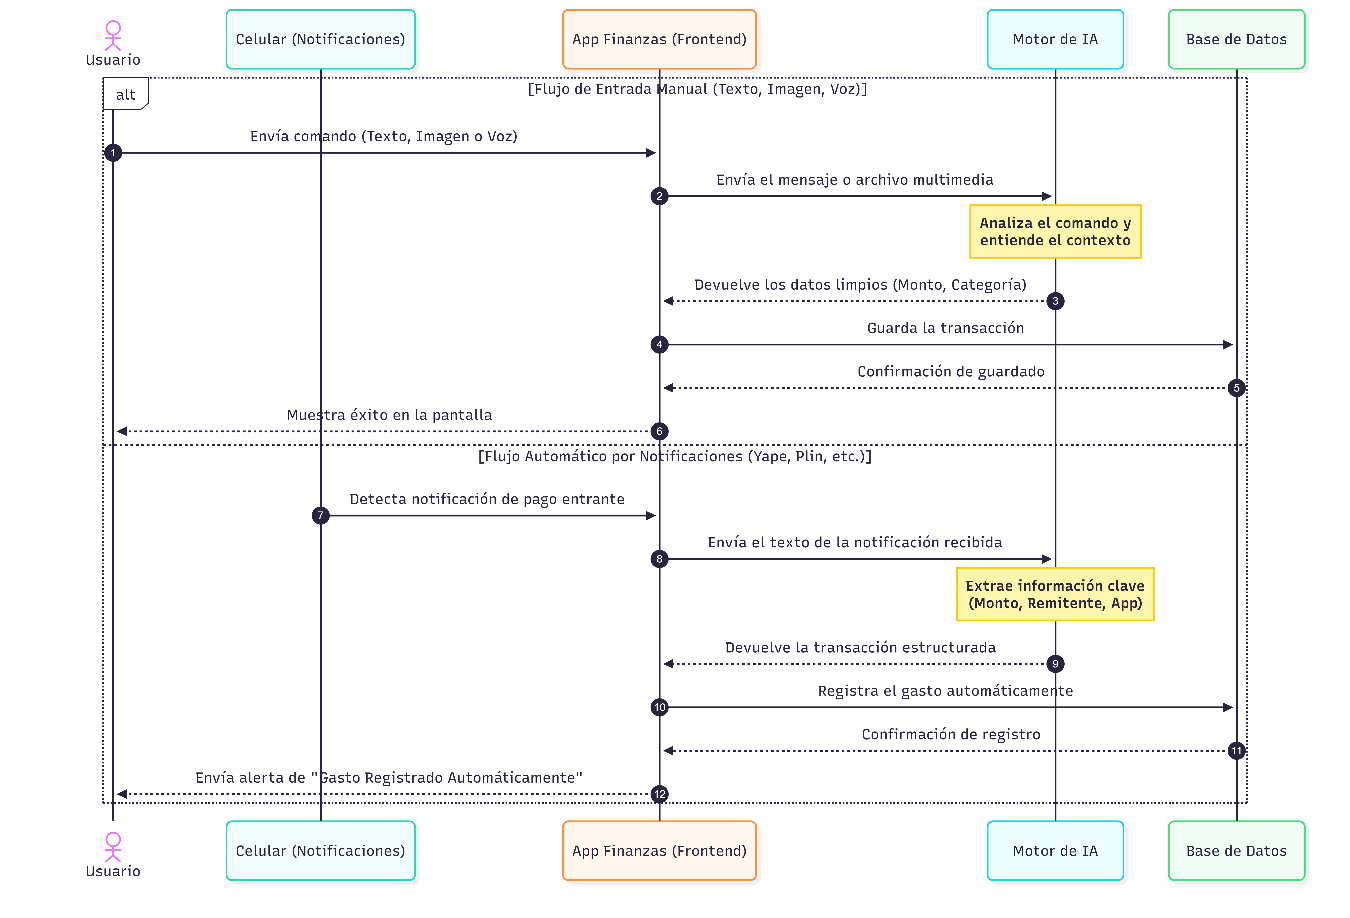
\includegraphics[width=0.7\textwidth]{flujo_actividades.png}
    \caption{Diagrama de Flujo de Actividades y Procesamiento del Software.}
    \label{fig:flujo_actividades}
\end{figure}

\newpage

% ==========================================
% ARQUITECTURA Y DISEÑO TÉCNICO DEL SISTEMA
% ==========================================
\section{ARQUITECTURA Y DISEÑO TÉCNICO DEL SISTEMA}

\subsection{Arquitectura General de la Aplicación}
La arquitectura de FinancIA! ha sido diseñada siguiendo un patrón cliente-servidor estructurado en capas desacopladas, lo que permite la modularidad del código y facilita la escalabilidad. El sistema consta de:
\begin{itemize}
    \item \textbf{Capa de Presentación (Frontend SPA):} Implementada en React 19, TypeScript y Vite. Gestiona el ciclo de vida de la interfaz de usuario, renderiza dinámicamente gráficos e indicadores del estado de ahorro y consume la API del servidor de manera asíncrona.
    \item \textbf{Capa de Manejo de Estado:} Zustand maneja la persistencia y distribución reactiva de la información financiera a través de la aplicación.
    \item \textbf{Capa de Servicio y Lógica de Negocio (Backend API):} Servidor Express que corre sobre Node.js. Administra la autenticación de usuarios, el procesamiento de las reglas de control de presupuestos y la orquestación inteligente de diálogos.
    \item \textbf{Capa de Persistencia:} SQLite utilizando la API nativa de Node.js v22 (`node:sqlite`). Se encarga de almacenar de manera estructurada los registros del usuario.
    \item \textbf{Servicio de Inteligencia Artificial:} Conector REST seguro con la API de Google Gemini para procesamiento de lenguaje natural y ejecución automática de comandos.
\end{itemize}

El despliegue de producción se unifica en el backend, el cual expone los servicios de la API REST e internamente sirve los archivos compilados del frontend (`dist/`), permitiendo una infraestructura de servidor único y simplificando el direccionamiento de red.

\subsection{Modelo de Datos y Esquema de Base de Datos}
La persistencia de FinancIA! se apoya en una base de datos relacional SQLite ligera y segura. Las relaciones están protegidas mediante restricciones de integridad y eliminaciones en cascada. A continuación se detallan las tablas y su esquema técnico:

\begin{enumerate}
    \item \textbf{users} (Usuarios):
    \begin{itemize}
        \item \textbf{email} (TEXT, PK): Correo electrónico único del usuario, normalizado en minúsculas.
        \item \textbf{name} (TEXT): Nombre completo del usuario.
        \item \textbf{initialized} (INTEGER): Bandera binaria (0 o 1) que indica si el usuario ya posee datos semillas por defecto (modo demo).
        \item \textbf{budget\_tips} (TEXT): Campo de texto largo que almacena las sugerencias de presupuestos generadas por la IA.
        \item \textbf{password} (TEXT): Contraseña de inicio de sesión (almacenada para validación en entorno seguro).
    \end{itemize}

    \item \textbf{transactions} (Transacciones):
    \begin{itemize}
        \item \textbf{id} (TEXT, PK): Identificador único autogenerado con el prefijo ``tx-''.
        \item \textbf{user\_email} (TEXT, FK): Correo del propietario de la transacción. Referencia a `users(email)` con eliminación en cascada (`ON DELETE CASCADE`).
        \item \textbf{merchant} (TEXT): Nombre del establecimiento o concepto del flujo (ej: Starbucks, Salario).
        \item \textbf{category} (TEXT): Nombre de la categoría de gasto o ingreso.
        \item \textbf{amount} (REAL): Monto numérico del movimiento en dólares estadounidenses.
        \item \textbf{date} (TEXT): Marca temporal o descripción relativa del registro (ej: ``Hoy'', ``Ayer'').
        \item \textbf{account} (TEXT): Tipo de cuenta o medio de pago (ej: ``Tarjeta Personal'', ``Efectivo'').
        \item \textbf{type} (TEXT): Clasificador del flujo (``expense'' o ``income'').
    \end{itemize}

    \item \textbf{budgets} (Presupuestos):
    \begin{itemize}
        \item \textbf{user\_email} (TEXT, FK): Propietario del presupuesto. Referencia a `users(email)` con `ON DELETE CASCADE`.
        \item \textbf{category} (TEXT): Categoría asociada al presupuesto.
        \item \textbf{spent} (REAL): Acumulado de gasto actual de la categoría.
        \item \textbf{limit\_val} (REAL): Límite financiero semanal establecido por el usuario.
        \item \textbf{icon} (TEXT): Identificador visual del icono a renderizar en la interfaz.
        \item \textbf{color} (TEXT): Código hexadecimal del color del presupuesto.
        \item \textbf{PRIMARY KEY} (user\_email, category).
    \end{itemize}

    \item \textbf{savings} (Metas de Ahorro):
    \begin{itemize}
        \item \textbf{user\_email} (TEXT, PK, FK): Referencia a `users(email)` con `ON DELETE CASCADE`.
        \item \textbf{name} (TEXT): Nombre de la meta de ahorro activa (ej: ``Fondo de Emergencia'').
        \item \textbf{target} (REAL): Monto objetivo a ahorrar en dólares.
        \item \textbf{current} (REAL): Balance actual acumulado en la meta.
        \item \textbf{recommendations} (TEXT): Sugerencias y análisis acumulados en formato Markdown.
    \end{itemize}

    \item \textbf{savings\_logs} (Historial de Depósitos a Ahorros):
    \begin{itemize}
        \item \textbf{id} (TEXT, PK): Identificador del registro con el prefijo ``sl-''.
        \item \textbf{user\_email} (TEXT, FK): Referencia a `users(email)` con `ON DELETE CASCADE`.
        \item \textbf{amount} (REAL): Monto depositado.
        \item \textbf{date} (TEXT): Fecha del depósito formatada.
        \item \textbf{note} (TEXT): Nota opcional descriptiva sobre la fuente del dinero ahorrado.
    \end{itemize}

    \item \textbf{chat\_messages} (Mensajería de Conversación):
    \begin{itemize}
        \item \textbf{id} (TEXT, PK): Identificador único de mensaje.
        \item \textbf{user\_email} (TEXT, FK): Referencia a `users(email)` con `ON DELETE CASCADE`.
        \item \textbf{chat\_id} (TEXT): Identificador de la sesión de chat activa.
        \item \textbf{sender} (TEXT): Emisor del mensaje (``user'' o ``ai'').
        \item \textbf{timestamp} (TEXT): Hora de envío del mensaje.
        \item \textbf{text} (TEXT): Contenido textual principal del mensaje.
        \item \textbf{transaction\_detail} (TEXT): Representación JSON serializada de los datos de la transacción en caso de que el mensaje registre un movimiento.
        \item \textbf{action\_chips} (TEXT): Array de botones rápidos serializados en JSON para interacciones de un clic (ej: ``Ver Estadísticas'').
        \item \textbf{info\_text} (TEXT): Alertas de presupuesto asociadas a la transacción.
    \end{itemize}
\end{enumerate}

\subsection{Orquestación de la Inteligencia Artificial e Integración de Gemini}
El motor de inteligencia artificial actúa como un agente autónomo conversacional que traduce lenguaje natural a operaciones de base de datos en tiempo real. 

\subsubsection{Inyección Dinámica de Contexto}
Para asegurar que el modelo posea conocimiento completo sobre el estado financiero actual del usuario antes de contestar, el backend extrae del motor SQLite los balances de ahorro, la lista de transacciones recientes y los límites de gasto de las categorías activas. Este resumen se inyecta dinámicamente en la directiva de sistema (\textit{System Instruction}) de la petición a la API de Gemini:

\begin{verbatim}
Aquí está el estado financiero actual del usuario:
- Ahorros: Meta: "Fondo de Emergencia" ($450.00 / $5000.00)
- Límites de Presupuesto: 
  * Comida fuera: Gastado $49.50 de un límite de $120.00
  * Transporte: Gastado $18.75 de un límite de $150.00
- Últimas Transacciones Registradas:
  * Gasto $45.00 en Green Cafe (Comida fuera, Hoy)
\end{verbatim}

\subsubsection{Declaración y Ejecución de Herramientas (Function Calling)}
El modelo de inteligencia artificial `gemini-3.5-flash` tiene declaradas tres herramientas nativas para interactuar con la base de datos de manera automatizada:
\begin{enumerate}
    \item \textbf{add\_transaction}: Permite añadir una transacción analizando variables clave extraídas del mensaje del usuario (`merchant`, `category`, `amount`, `type`, `account`).
    \item \textbf{deposit\_savings}: Ejecuta aportes monetarios a la meta de ahorro actual especificando el monto y el concepto.
    \item \textbf{update\_budget\_limit}: Modifica el presupuesto semanal de una categoría específica.
\end{enumerate}

Cuando el usuario envía un texto, el servidor procesa el mensaje inicial. Si Gemini decide llamar a una herramienta, devuelve un objeto de llamada de función (`functionCall`). El backend intercepta la llamada, realiza la consulta correspondiente a la base de datos SQLite y devuelve el resultado a la API de Gemini en una segunda vuelta. El modelo de lenguaje analiza el resultado de la base de datos y genera una respuesta final amigable y empática en lenguaje natural.

\subsection{Manejo del Estado Global en el Frontend (Zustand)}
El frontend utiliza el gestor de estados ligero Zustand para centralizar y coordinar las peticiones a la API del backend, manteniendo sincronizada la interfaz reactiva sin provocar ciclos de renderizado innecesarios.

El estado del cliente está estructurado en dos almacenes principales:
\begin{itemize}
    \item \textbf{useAuthStore}: Controla el estado de sesión (`user`, `isAuthenticated`), gestiona las peticiones de registro, inicio de sesión y cambio de contraseña, y almacena las credenciales locales de sesión mediante la persistencia automatizada en `localStorage` del navegador.
    \item \textbf{useFinancesStore}: Administra toda la información financiera y conversacional (`transactions`, `budgets`, `savings`, `chatHistory`, `categories`). Proporciona acciones como `sendMessage`, la cual envía el mensaje del usuario al backend y, tras recibir la respuesta, actualiza el estado de las transacciones y presupuestos en un solo ciclo de renderizado.
\end{itemize}

\subsection{Contrato de Servicios y API Endpoints}
El backend expone un conjunto de endpoints RESTful bajo el prefijo `/api` protegidos por una cabecera de autenticación personalizada (`x-user-email`):

\begin{table}[H]
\centering
\singlespacing
\caption{Endpoints y Especificaciones del Servidor REST Backend}
\label{tab:endpoints}
\footnotesize
\begin{tabular}{p{1.8cm}p{4.4cm}p{3.8cm}p{4.5cm}}
\toprule
\textbf{Método} & \textbf{Ruta de la API} & \textbf{Cuerpo / Parámetros} & \textbf{Respuesta Esperada} \\
\midrule
POST & /api/auth/login & \{email, password\} & \{success: true, user\} \\
\addlinespace
POST & /api/auth/register & \{name, email, password\} & \{success: true, user\} \\
\addlinespace
PUT & /api/auth/change-password & \{currentPassword, newPassword\} & \{success: true, message\} \\
\addlinespace
GET & /api/finances & Header: x-user-email & \{success: true, state\} \\
\addlinespace
GET & /api/finances/chat-history & ?chatId & \{success: true, chatHistory\} \\
\addlinespace
POST & /api/finances/chat & \{text, chatId\} & \{success: true, response, state\} \\
\addlinespace
POST & /api/finances/chat/new-with-prompt & \{type, customPrompt\} & \{success: true, chatId, state\} \\
\addlinespace
GET / POST & /api/finances/transactions & POST: \{merchant, category, amount, type\} & GET: \{success: true, transactions\} \newline POST: \{success: true, transaction, state\} \\
\addlinespace
GET / PUT / DELETE & /api/finances/transactions/:id & PUT: Campos a actualizar \newline (Parámetro ID en URL) & GET: \{success: true, transaction\} \newline PUT/DELETE: \{success: true, state\} \\
\addlinespace
PUT & /api/finances/budgets & \{category, limit, spent\} & \{success: true, state\} \\
\addlinespace
PUT / DELETE & /api/finances/savings & PUT: \{name, target, start\_date, deadline\} & \{success: true, state\} \\
\addlinespace
GET & /api/finances/savings/history & Ninguno & \{success: true, history\} \\
\addlinespace
POST / PUT / DELETE & /api/finances/categories & POST: \{name\} \newline PUT: \{oldName, newName\} \newline DELETE: ?name & \{success: true, state\} \\
\addlinespace
POST / DELETE & /api/finances/chat-messages & POST: \{message, chatId\} \newline DELETE: ?chatId & \{success: true, state\} \\
\addlinespace
DELETE & /api/finances/chat-messages/:id & Parámetro ID en URL & \{success: true, state\} \\
\addlinespace
PUT & /api/finances/chat-messages/:id/remove-action-chips & Parámetro ID en URL & \{success: true, state\} \\
\addlinespace
DELETE & /api/finances/account & Ninguno & \{success: true\} \\
\bottomrule
\end{tabular}
\end{table}

\newpage

% ==========================================
% MANUAL DE INSTALACIÓN, CONFIGURACIÓN Y EJECUCIÓN
% ==========================================
\section{MANUAL DE INSTALACIÓN, CONFIGURACIÓN Y EJECUCIÓN}

\subsection{Requisitos Previos del Sistema}
Para asegurar el correcto funcionamiento del servidor local de FinancIA! es indispensable contar con:
\begin{itemize}
    \item \textbf{Node.js} versión 22.5.0 o superior (requisito de runtime obligatorio para dar soporte a la funcionalidad nativa de base de datos `node:sqlite`).
    \item Gestor de dependencias \textbf{npm} (integrado por defecto con Node.js).
    \item Una clave de API válida de Google Gemini obtenida a través de Google AI Studio.
\end{itemize}

\subsection{Configuración de Variables de Entorno}
En la raíz de la carpeta `backend`, cree un archivo `.env` tomando como base el archivo `.env.example` y configure los siguientes parámetros:
\begin{verbatim}
PORT=3000
GEMINI_API_KEY=su_clave_de_api_de_gemini
DATABASE_PATH=./data/finances.db
CORS_ORIGIN=http://localhost:5173
\end{verbatim}

\subsection{Ejecución en Entorno de Desarrollo}
Para realizar pruebas de código o modificaciones con recarga rápida (HMR), se deben inicializar el backend y el frontend por separado:
\begin{enumerate}
    \item \textbf{Levantar el Servidor REST (Backend):}
    \begin{verbatim}
    cd backend
    npm install
    npm run dev
    \end{verbatim}
    El servidor backend quedará escuchando peticiones en el puerto `http://localhost:3000`.

    \item \textbf{Iniciar la Aplicación de React (Frontend):}
    \begin{verbatim}
    cd ../frontend
    npm install
    npm run dev
    \end{verbatim}
    Esto levantará el servidor de desarrollo de Vite en la dirección `http://localhost:5173`.
\end{enumerate}

\subsection{Ejecución en Modo Producción (Servidor Único)}
Para entornos de despliegue consolidado que sirvan la aplicación desde un puerto único, ejecute la compilación del proyecto:
\begin{enumerate}
    \item \textbf{Compilar la SPA de React:}
    \begin{verbatim}
    cd frontend
    npm install
    npm run build
    \end{verbatim}
    Esto empaquetará todo el código en el directorio estático `frontend/dist`.

    \item \textbf{Levantar el Servidor Unificado:}
    \begin{verbatim}
    cd ../backend
    npm install
    npm run start
    \end{verbatim}
    El servidor Express servirá la base de datos, responderá a la API en `/api/*` y servirá el frontend de React directamente en el puerto configurado (por defecto `http://localhost:3000`), sin necesidad de configurar un proxy o servidor web externo.
\end{enumerate}

\newpage

% ==========================================
% EARLY ADOPTERS
% ==========================================
\section{EARLY ADOPTERS}

De acuerdo con las especificaciones del diseño del proyecto, en la Tabla \ref{tab:early_adopters} se presenta la caracterización de los usuarios seleccionados como \textit{early adopters} para las pruebas de usabilidad y validación del MVP. Cada perfil ha sido seleccionado estratégicamente para evaluar la reducción de fricción en diferentes hábitos de gestión financiera.

\begin{table}[H]
\centering
\singlespacing
\caption{Perfil y Justificación de los Early Adopters del MVP}
\label{tab:early_adopters}
\begin{tabular}{p{3.5cm}p{5.7cm}p{6cm}}
\toprule
\textbf{Usuario} & \textbf{Perfil} & \textbf{Justificación} \\
\midrule
Usuario 1 \newline José L. Mariño & Estudiante de pregrado (22 años, M). Usuario de BCP y Yape. Experimenta frustración por la falta de categorización inteligente y por realizar sumas manuales de microgastos cotidianos. & Representa al segmento estudiantil nativo digital que maneja múltiples microgastos diarios. Útil para validar la categorización inteligente y la reducción de fricción al registrar datos. \\
\addlinespace
Usuario 2 \newline Jean P. Pinedo & Trabajador independiente / Freelancer (22 años, M). Combina apps bancarias con Excel manual. Frustrado por el tiempo que quita el registro manual y la lentitud de balance de cuentas. & Representa a trabajadores independientes que requieren optimizar su tiempo diario. Permite evaluar la rapidez y centralización de balances financieros inmediatos. \\
\addlinespace
Usuario 3 \newline Frank H. Bustillos & Estudiante de pregrado (23 años, M). Usuario de Yape. Frustrado por la gestión fragmentada al no poder consolidar movimientos de múltiples tarjetas de otros bancos. & Clave para validar la necesidad de centralización de balances generales y probar la usabilidad de la interfaz conversacional para consolidar gastos diversos. \\
\addlinespace
Usuario 4 \newline Augusto Arias & Estudiante de pregrado (22 años, M). No utiliza ninguna aplicación de control financiero por considerarlas sumamente lentas, tediosas y con formularios extensos y complejos. & Representa al perfil escéptico que rechaza las herramientas financieras tradicionales. Permite evaluar si el canal conversacional con IA elimina la barrera de adopción. \\
\addlinespace
Usuario 5 \newline Jennifer Esquivel & Emprendedora / Comerciante (38 años, F). Usuaria de la app de Banco de la Nación. Frustrada por la interfaz obsoleta, inicio lento y falta de gráficos para sus metas de ahorro. & Aporta la perspectiva de un perfil de mayor edad y orientación comercial que busca planificar metas específicas de ahorro y demanda una visualización interactiva y estimulante. \\
\bottomrule
\end{tabular}
\end{table}

\newpage

% ==========================================
% VALIDACIÓN DEL MVP
% ==========================================
\section{VALIDACIÓN DEL MVP}

\subsection{Metodología}
La validación del MVP se estructuró para evaluar la usabilidad, la fricción del usuario y el cumplimiento del objetivo principal del sistema mediante un cuestionario estandarizado.
\begin{itemize}
    \item \textbf{Fecha de prueba:} Las sesiones de prueba y recolección de encuestas se desarrollaron del 2 de julio al 6 de julio de 2025.
    \item \textbf{Número de usuarios:} Se evaluó a una muestra de 5 usuarios seleccionados bajo los perfiles de early adopters del sistema.
    \item \textbf{Actividades realizadas:}
    \begin{enumerate}
        \item \textit{Fase de inducción y perfilado:} Se registró la información demográfica (edad, sexo) y de hábitos financieros de cada participante para contextualizar su perfil.
        \item \textit{Test de interacción con el MVP:} Los usuarios interactuaron libremente con el chatbot conversacional para registrar gastos en lenguaje natural, y navegaron por los módulos de historial, límites presupuestarios y metas de ahorro.
        \item \textit{Aplicación de la encuesta de validación:} Al finalizar las pruebas, cada usuario completó el cuestionario estructurado en la plataforma Microsoft Forms para evaluar cuantitativamente y cualitativamente las funcionalidades.
    \end{enumerate}
\end{itemize}

\subsection{Resultados}
Los resultados cuantitativos y cualitativos obtenidos a partir del cuestionario aplicado a los 5 participantes se presentan en la Tabla \ref{tab:resultados_validacion}.

\begin{table}[H]
\centering
\caption{Resultados de la Encuesta y Cuestionario de Validación del MVP}
\label{tab:resultados_validacion}
\begin{tabular}{p{5.5cm}p{9.3cm}}
\toprule
\textbf{Pregunta / Métrica Clave} & \textbf{Resultado y Análisis de Datos} \\
\midrule
¿Usa actualmente alguna aplicación de seguimiento financiero? & El 80\% (4 de 5) utiliza herramientas móviles. El 20\% no cuenta con ninguna herramienta de control. \\
\addlinespace
¿El registro por chat e IA redujo la fatiga de la digitación manual? & El 100\% indicó que la interfaz conversacional resolvió con éxito la fricción y pereza de la entrada tradicional de datos. \\
\addlinespace
Nivel de facilidad de uso del chatbot de IA y navegación general (1-5) & Se obtuvo una calificación promedio de \textbf{4.6 / 5.0} (92\% de satisfacción), destacando la claridad y la inmediatez. \\
\addlinespace
Utilidad de la visualización de presupuestos mediante semáforos & El 80\% lo calificó como muy intuitivo para el control diario. El 20\% sugirió presentarlo de otra forma. \\
\addlinespace
Nivel de utilidad del módulo de metas de ahorro (Escala 1-5) & Se obtuvo un promedio de \textbf{4.4 / 5.0}, valorando el simulador de depósitos rápidos y la configuración de reportes de IA. \\
\addlinespace
Requerimientos de seguridad indispensables elegidos por los usuarios & El 60\% prefiere autenticación biométrica (huella/Face ID) y el 40\% prefiere verificación en dos pasos (2FA/SMS). \\
\addlinespace
Probabilidad de adoptar la app como herramienta principal (0-10) & Puntuación promedio de \textbf{8.4 / 10}. El 100\% de los usuarios valoró la probabilidad con 8 o más, mostrando alta intención de uso. \\
\bottomrule
\end{tabular}
\end{table}

\subsection{Evidencias de Validación}
Como soporte de las pruebas de validación realizadas, las respuestas individuales fueron consolidadas y registradas digitalmente. El diseño del cuestionario de validación y el acceso al formulario de recolección oficial se encuentran referenciados detalladamente en el \textbf{Anexo B} de este informe. Asimismo, el detalle individualizado de las respuestas cualitativas de cada evaluador se encuentra organizado en las bitácoras de respuestas del entregable.

\newpage

% ==========================================
% RETROALIMENTACIÓN Y MEJORAS
% ==========================================
\section{RETROALIMENTACIÓN Y MEJORAS}

En la Tabla \ref{tab:retroalimentacion_mejoras} se detallan los datos recolectados de cada uno de los cinco early adopters durante las pruebas de usabilidad y su respectiva propuesta de mejora para el sistema.

\begin{table}[H]
\centering
\singlespacing
\caption{Retroalimentación de Usuarios y Propuestas de Mejora del MVP}
\label{tab:retroalimentacion_mejoras}
\begin{tabular}{p{3.5cm}p{5.8cm}p{5.9cm}}
\toprule
\textbf{Early Adopter} & \textbf{Observación Realizada} & \textbf{Mejora Propuesta} \\
\midrule
Usuario 1 \newline José L. Mariño & Observó que las categorías de presupuesto predefinidas son fijas. Desea agrupar gastos de fotocopias o libros en una categoría específica de ``Educación''. & Permitir la creación y edición de categorías de gasto personalizadas a través de comandos de chat o en la interfaz de Límites. \\
\addlinespace
Usuario 2 \newline Jean P. Pinedo & La interfaz de chat es rápida y cómoda, pero desearía un recordatorio semanal proactivo sobre el estado del presupuesto sin tener que ingresar a la app. & Diseñar un sistema de notificaciones externas de la IA (vía Telegram o correo electrónico) con resúmenes de rendimiento. \\
\addlinespace
Usuario 3 \newline Frank H. Bustillos & Al cometer un error de escritura en el chat (ej. poner un cero de más), no pudo corregirlo directamente en la ventana de conversación. & Implementar un botón de ``Deshacer'' (\textit{Undo}) o edición rápida en la misma tarjeta generada por el chat. \\
\addlinespace
Usuario 4 \newline Augusto Arias & Registrar manualmente o por chat cada gasto del negocio resulta demandante. Considera vital la sincronización bancaria automática. & Desarrollar integraciones con APIs de banca abierta (\textit{Open Banking}) para sincronización de saldos y movimientos bancarios. \\
\addlinespace
Usuario 5 \newline Jennifer Esquivel & El simulador de ahorros incrementa el total acumulado, pero se pierde el registro cronológico de los depósitos ficticios ingresados. & Crear una pestaña de ``Historial de Depósitos'' en el módulo de Ahorros para listar montos y fechas de aportaciones a metas. \\
\bottomrule
\end{tabular}
\end{table}

\newpage

% ==========================================
% CONCLUSIONES Y TRABAJO FUTURO
% ==========================================
\section{CONCLUSIONES Y TRABAJO FUTURO}

\subsection{Conclusiones del Diagnóstico del Problema}
\begin{itemize}
    \item \textbf{Fricción del registro manual como causa raíz:} Se identificó que la incomodidad del registro manual es la causa raíz de la desorganización financiera de la comunidad universitaria, superando a la falta de ingresos por sí misma, ya que el esfuerzo cognitivo requerido compite con el tiempo de estudio y descanso.
    \item \textbf{Impacto transversal y choque de autonomía:} El desbalance financiero afecta de forma transversal en la UNAS, pero se manifiesta con severidad crítica en los estudiantes nuevos debido a su falta de experiencia previa gestionando presupuestos de manera autónoma lejos de sus hogares.
    \item \textbf{Oportunidad tecnológica:} Existe una oportunidad tecnológica clara para desarrollar una herramienta digital inteligente que elimine el registro manual, integrándose de forma orgánica en la rutina diaria de los usuarios mediante entradas conversacionales.
\end{itemize}

\subsection{Conclusiones del Diseño Visual y Arquitectura}
\begin{itemize}
    \item \textbf{Valor del canal conversacional:} La implementación de una barra de captura conversacional y multimodal (texto, audio y simulación de imagen) constituye el principal valor del sistema FinancIA!, al delegar la carga cognitiva de la entrada de datos a la inteligencia artificial de Gemini.
    \item \textbf{Modularidad y sincronización reactiva:} La clara separación arquitectónica entre el panel lateral de métricas (Analytics) y la vista principal de transacciones permite una sincronización reactiva en tiempo real del estado global en el cliente (Zustand) tras procesar cada gasto en el backend (SQLite y Express).
    \item \textbf{Usabilidad responsiva:} El diseño responsivo que transforma el panel lateral fijo en escritorio a un menú lateral deslizable en móvil, junto con la disposición inferior de los controles de captura, garantiza una usabilidad óptima adaptada al contexto de movilidad de los estudiantes.
    \item \textbf{Curva de aprendizaje nula:} El uso del \textit{Empty State} en el Dashboard inicial y un diseño minimalista dirigen la atención visual del usuario de manera inmediata a la acción de registro, garantizando una curva de adopción prácticamente nula.
\end{itemize}

\subsection{Conclusiones de la Validación del MVP}
\begin{itemize}
    \item \textbf{Reducción de fatiga en el registro:} La validación del MVP demuestra que la adopción de interfaces conversacionales y procesamiento de lenguaje natural simplifica dramáticamente el registro de transacciones, reduciendo la fricción principal que causa el abandono de las aplicaciones de finanzas personales tradicionales.
    \item \textbf{Efectividad de indicadores gamificados:} La incorporación de elementos visuales dinámicos de semaforización presupuestaria y barras de progreso para el ahorro promueve el autocontrol del gasto y facilita una lectura rápida del estado financiero, logrando una excelente aceptación por parte del grupo de early adopters (4.6/5.0 de satisfacción general).
    \item \textbf{Guía para el desarrollo comercial futuro:} La retroalimentación detallada provista por los early adopters constituye una guía clara de prioridades de desarrollo para futuras iteraciones de producto, destacando la necesidad de incorporar flujos de corrección ágiles, categorías configurables y la automatización mediante la conexión a cuentas bancarias del usuario.
\end{itemize}

\subsection{Trabajo Futuro}
Para la evolución del sistema FinancIA! en fases comerciales posteriores, se proponen las siguientes directrices técnicas basadas en los requerimientos recogidos:
\begin{itemize}
    \item \textbf{Sincronización mediante Open Banking:} Desarrollar adaptadores de APIs bancarias bajo el estándar internacional de finanzas abiertas para sincronizar de manera pasiva y segura los saldos del usuario y eliminar por completo la carga de registro de transacciones ordinarias.
    \item \textbf{Mejora en la Edición Conversacional:} Implementar un sistema de control de historial en las respuestas del chat, permitiendo deshacer transacciones creadas de forma errónea por la IA directamente mediante comandos de texto rápidos (ej: ``cancela el último gasto'') o a través de tarjetas interactivas de edición rápida.
    \item \textbf{Motor de Canales de Alerta Externos:} Ampliar el alcance de las notificaciones proactivas de la IA diseñando webhooks para integrar asistentes robotizados en plataformas de comunicación cotidianas como Telegram o WhatsApp, permitiendo al usuario registrar transacciones y recibir resúmenes directamente desde su aplicación de chat preferida.
    \item \textbf{Historiales de Metas de Ahorro Completos:} Refactorizar el módulo de metas de ahorro para permitir historiales de depósitos con control temporal y gráficos interactivos de proyección de ahorros a largo plazo basados en simulaciones heurísticas.
\end{itemize}

\newpage

% ==========================================
% ANEXOS
% ==========================================
\section{ANEXOS}

\subsection{Anexo A: Evidencias Gráficas del MVP}
En esta sección se presentan las capturas de pantalla de la interfaz de usuario web interactiva desarrollada para el MVP del sistema FinancIA!:

\begin{figure}[H]
    \centering
    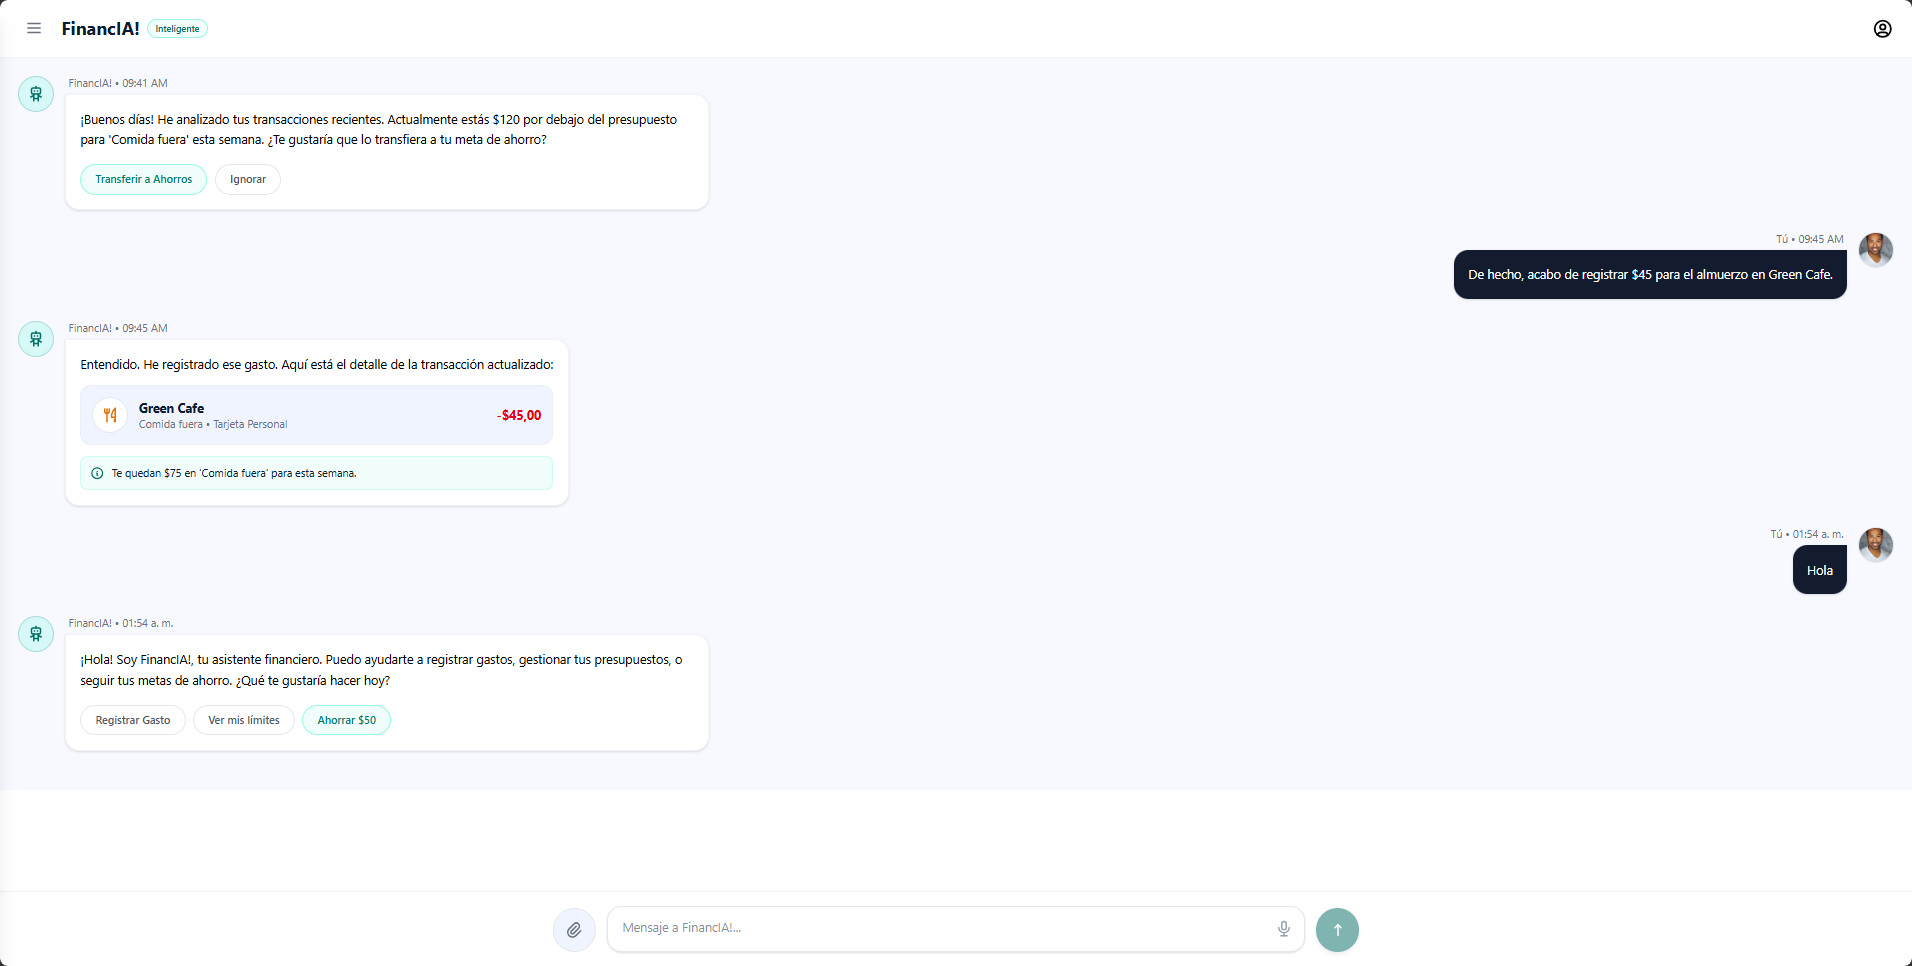
\includegraphics[width=0.85\textwidth]{chat_screenshot.png}
    \caption{Interfaz del Chat con Asistente de IA para el Registro Conversacional.}
    \label{fig:chat_ia}
\end{figure}

\begin{figure}[H]
    \centering
    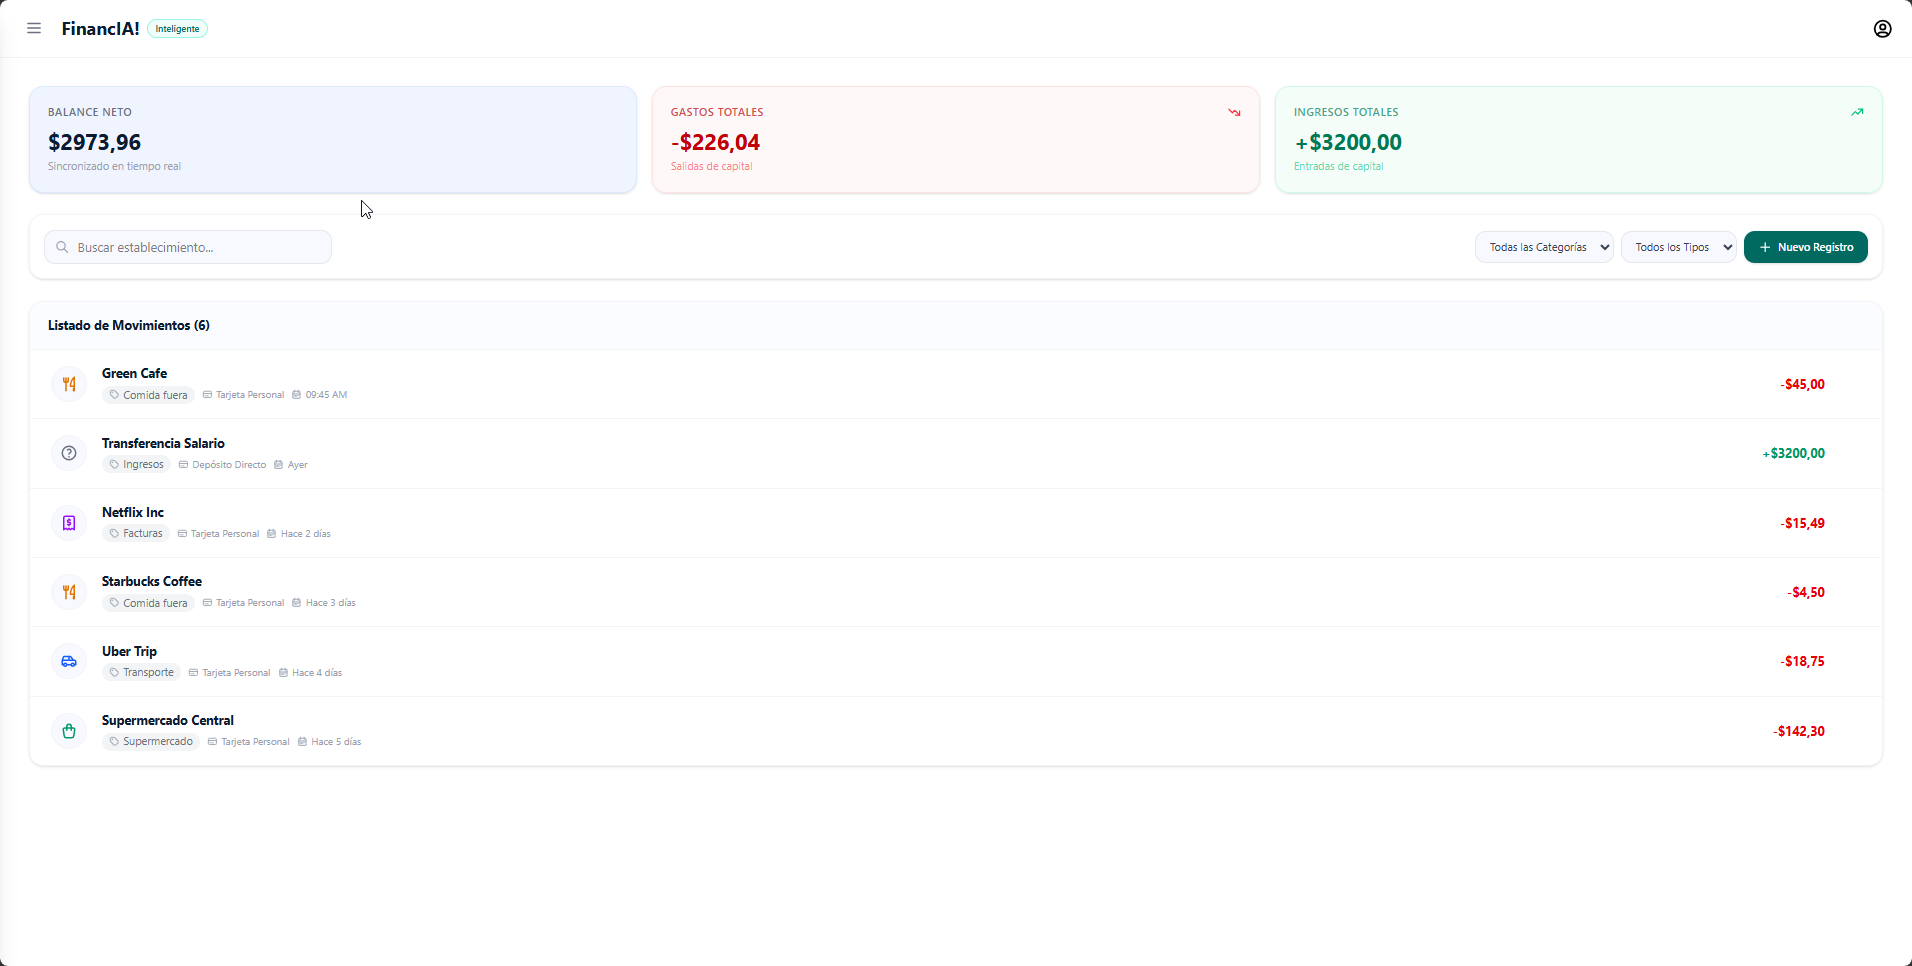
\includegraphics[width=0.85\textwidth]{movimientos_screenshot.png}
    \caption{Historial de Movimientos y Visualizador de Balances Generales.}
    \label{fig:movimientos}
\end{figure}

\begin{figure}[H]
    \centering
    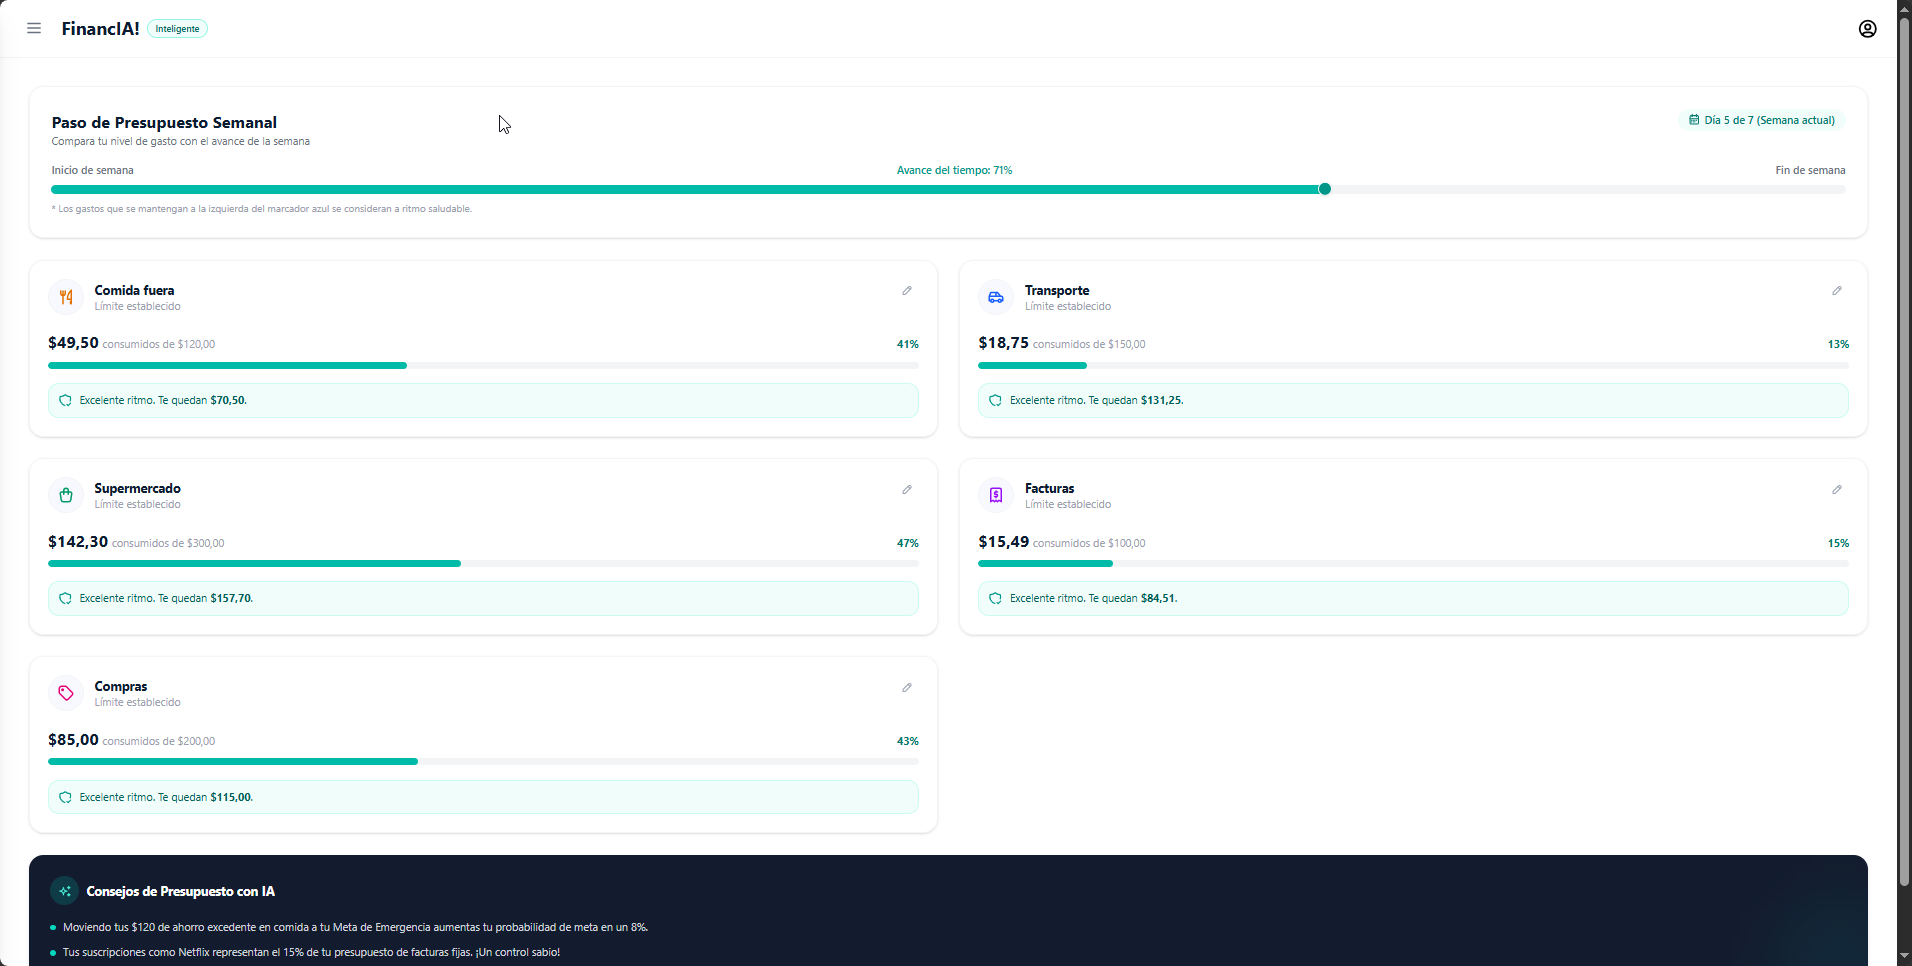
\includegraphics[width=0.85\textwidth]{limites_screenshot.png}
    \caption{Panel de Control de Presupuestos y Progreso Semanal.}
    \label{fig:limites}
\end{figure}

\begin{figure}[H]
    \centering
    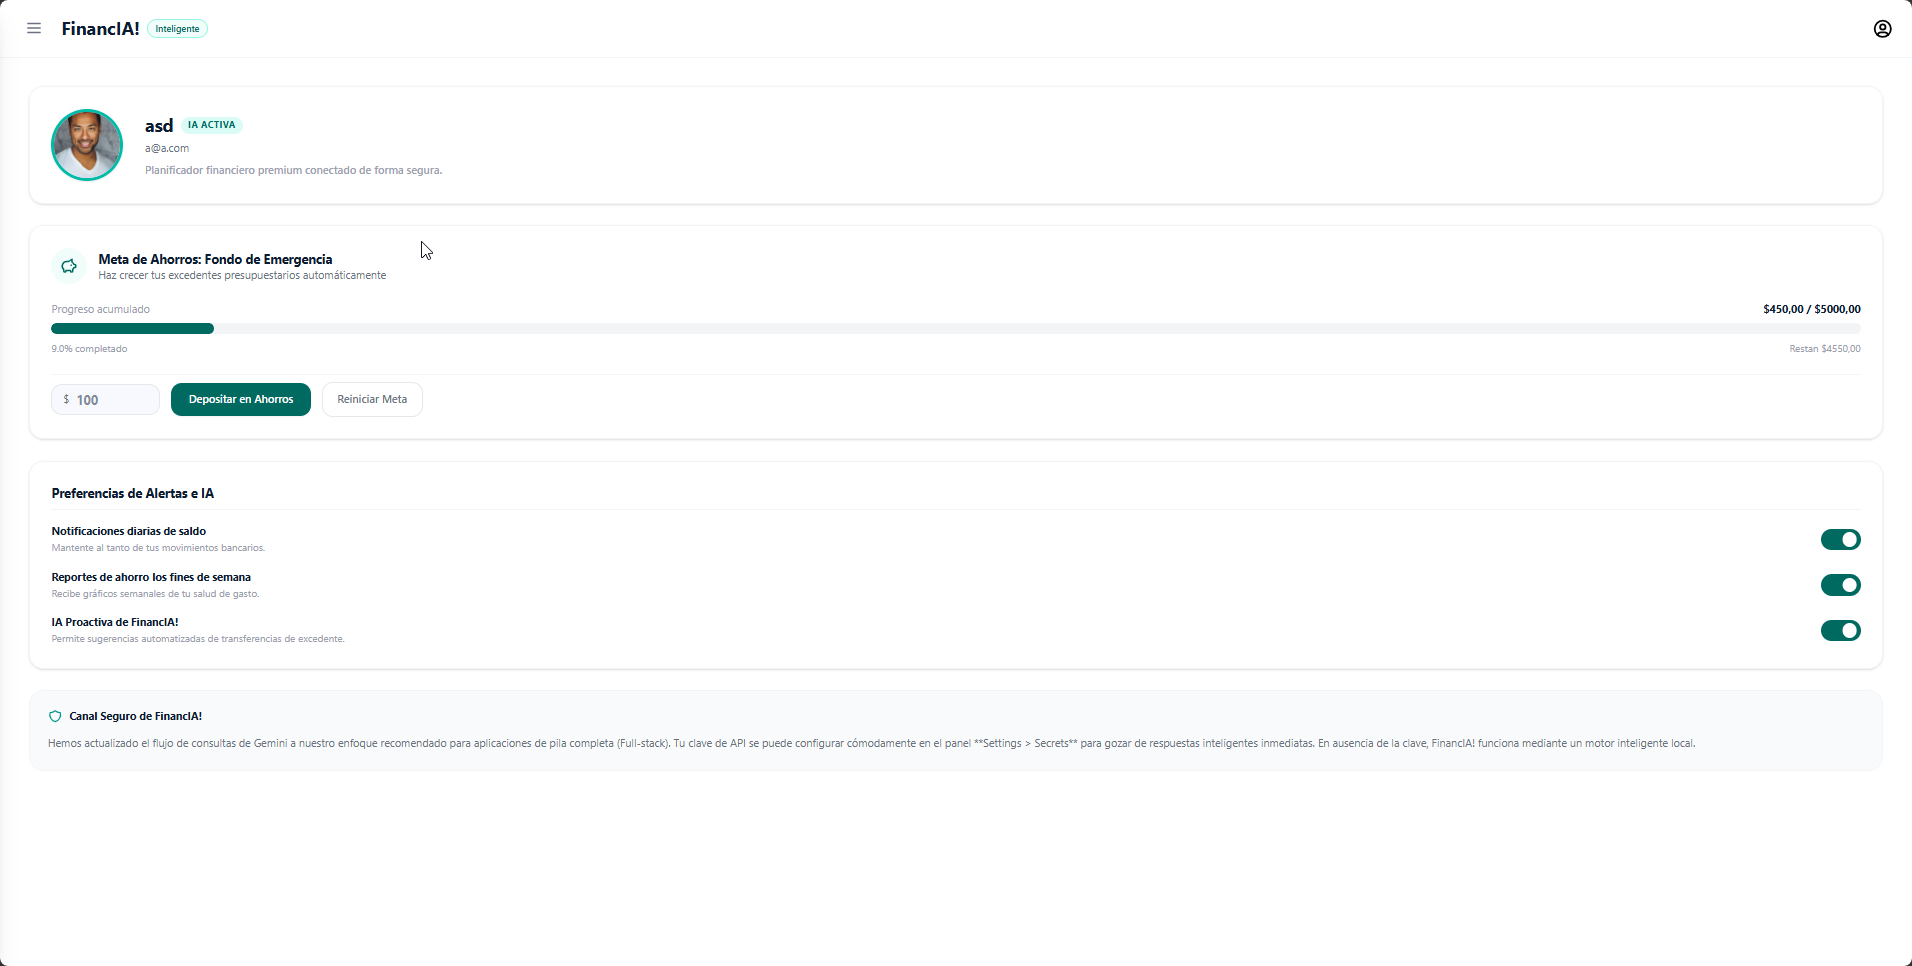
\includegraphics[width=0.85\textwidth]{ahorros_screenshot.png}
    \caption{Módulo de Metas de Ahorro y Configuración de Alertas.}
    \label{fig:ahorros}
\end{figure}

\newpage

\subsection{Anexo B: Prototipo de Alta Fidelidad en Figma (Diseño Conceptual Inicial)}
En esta sección se presentan las capturas del prototipo interactivo de alta fidelidad diseñado inicialmente en Figma durante la fase de concepción de la solución (Entregable 2):

\begin{figure}[H]
    \centering
    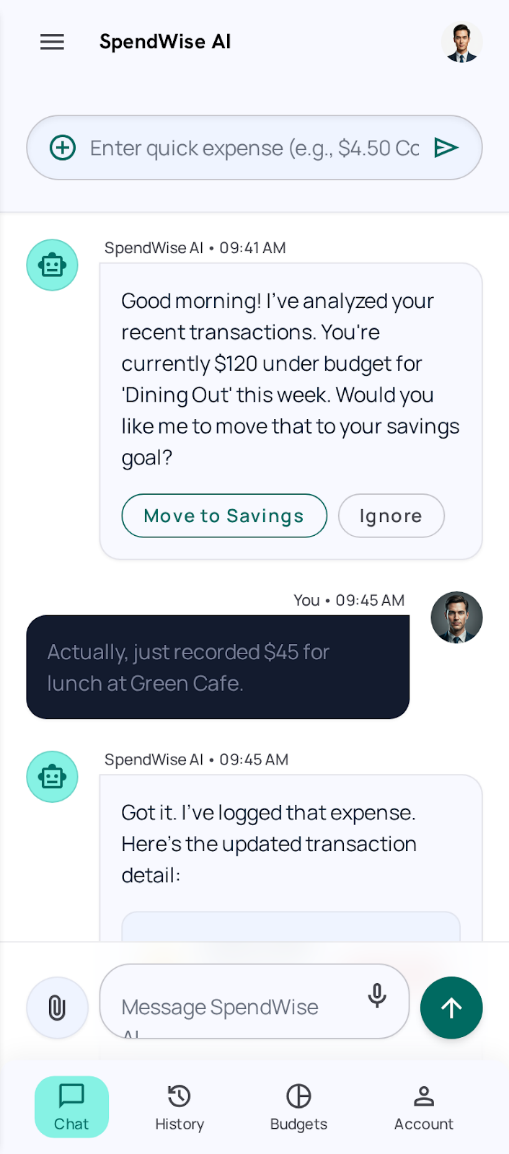
\includegraphics[width=0.45\textwidth]{figma_chat_movil.png}
    \caption{Prototipo de Figma: Vista de chat para dispositivos móviles.}
    \label{fig:figma_chat_movil}
\end{figure}

\begin{figure}[H]
    \centering
    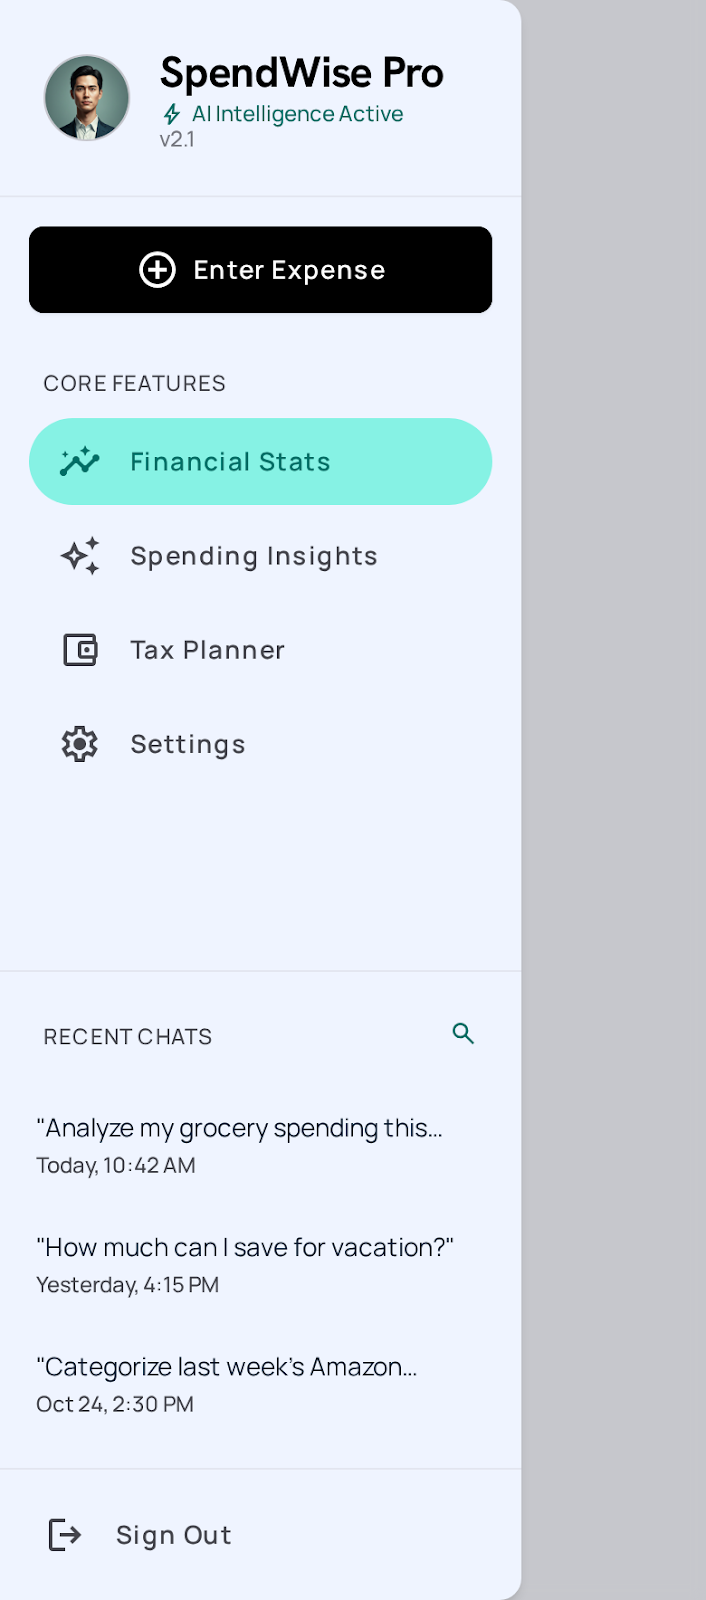
\includegraphics[width=0.45\textwidth]{figma_sidebar_movil.png}
    \caption{Prototipo de Figma: Vista de la barra lateral para dispositivos móviles.}
    \label{fig:figma_sidebar_movil}
\end{figure}

\begin{figure}[H]
    \centering
    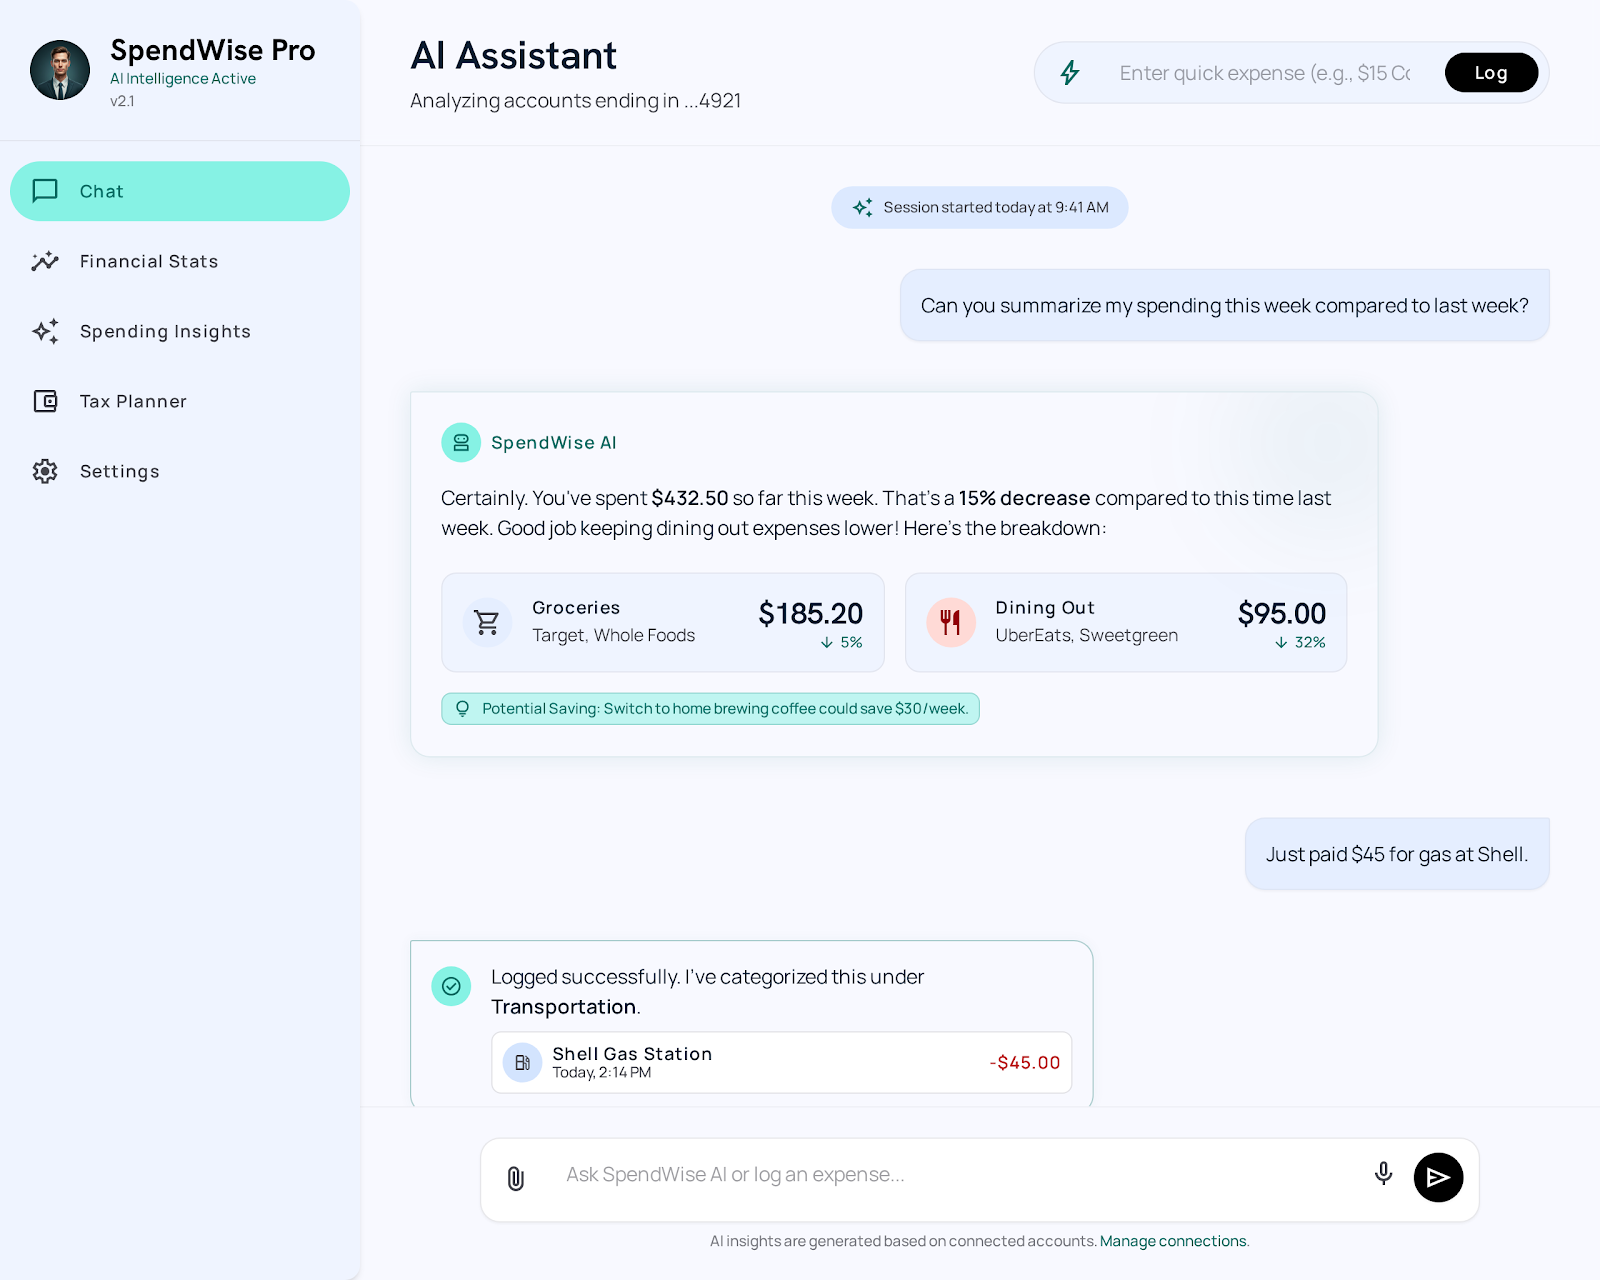
\includegraphics[width=0.85\textwidth]{figma_chat_desktop.png}
    \caption{Prototipo de Figma: Vista de chat para dispositivos de escritorio.}
    \label{fig:figma_chat_desktop}
\end{figure}

\begin{figure}[H]
    \centering
    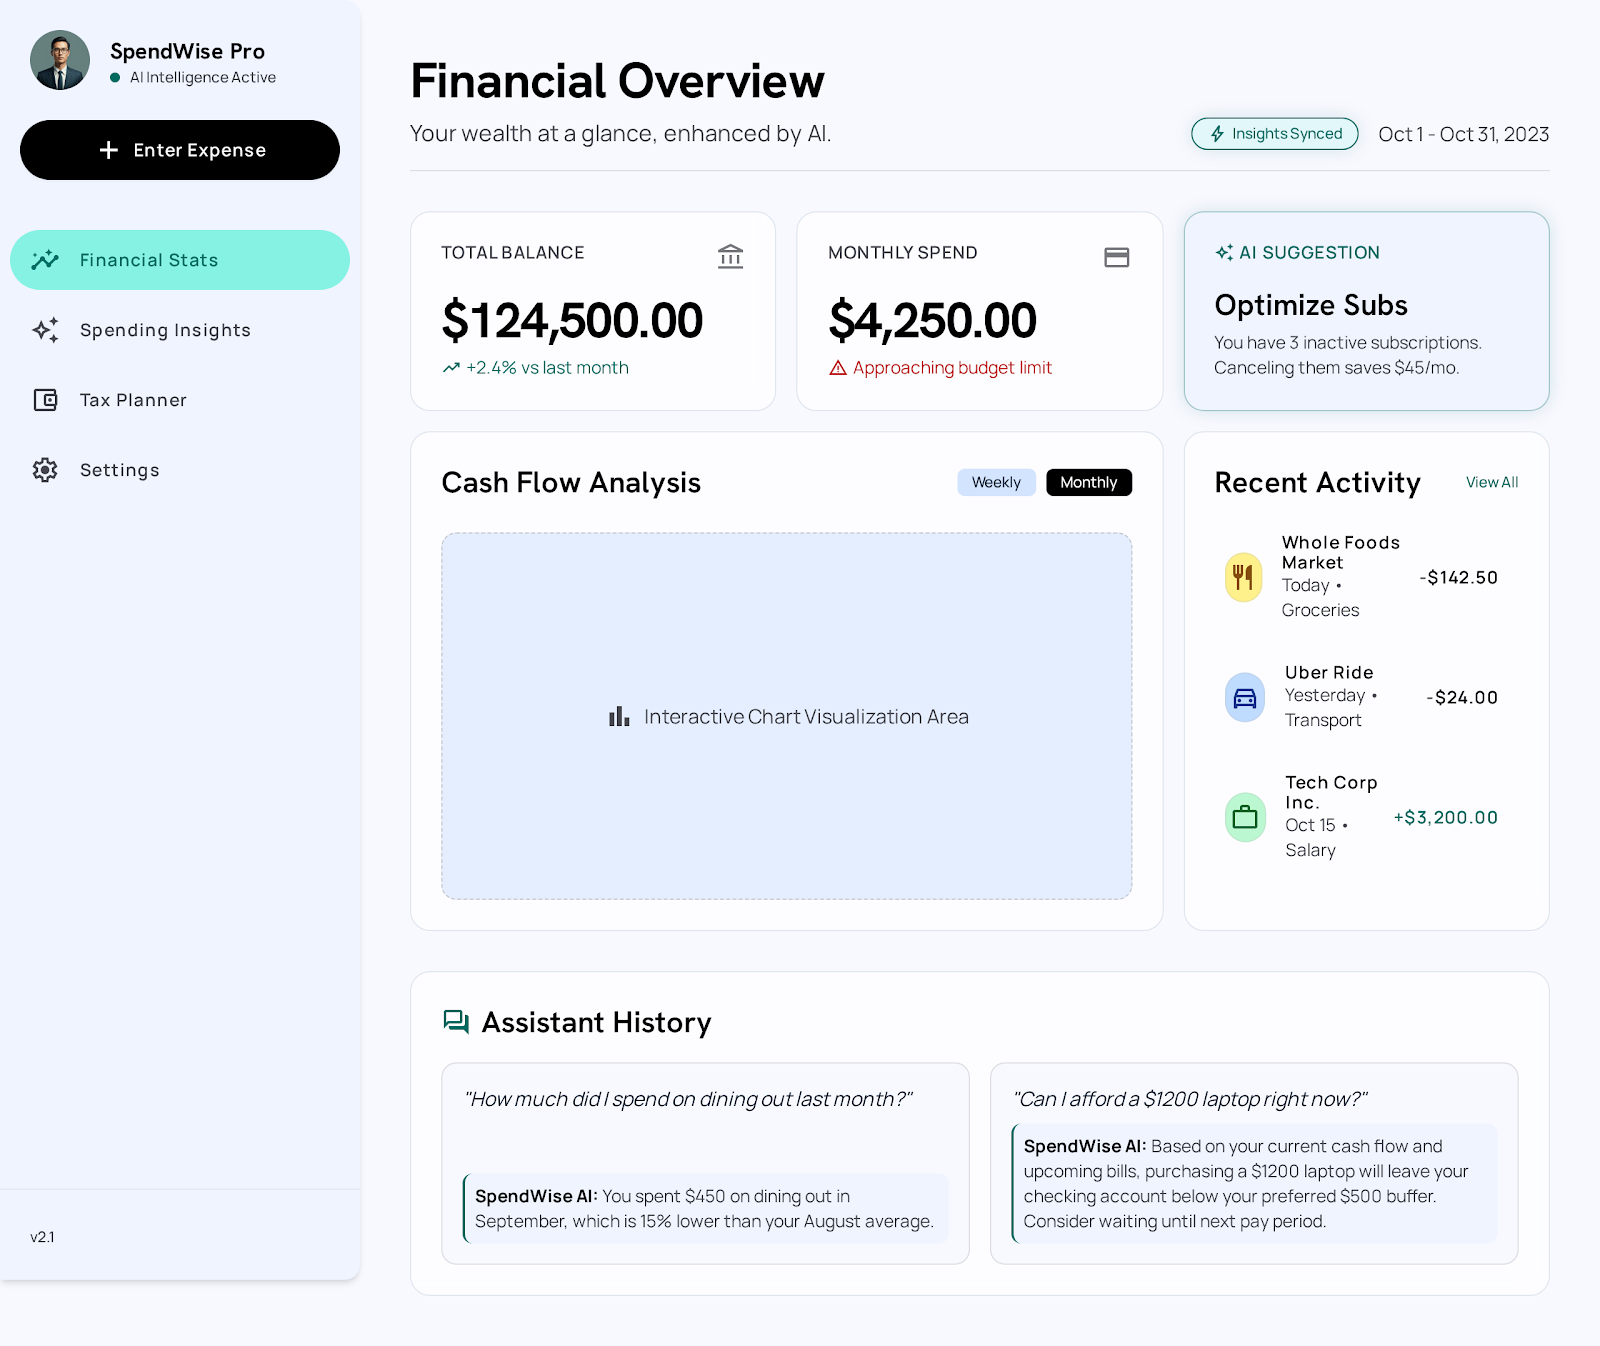
\includegraphics[width=0.85\textwidth]{figma_stats_desktop.png}
    \caption{Prototipo de Figma: Vista de estadísticas para dispositivos de escritorio.}
    \label{fig:figma_stats_desktop}
\end{figure}

\newpage

\subsection{Anexo C: Enlaces de Acceso y Recursos del Proyecto}

\textbf{Diseño y Estructura del Formulario de Validación:} \\
El cuestionario de validación utilizado para evaluar y recopilar la retroalimentación de los \textit{early adopters} puede ser consultado en el siguiente enlace oficial de Microsoft Forms: \\
\url{https://forms.cloud.microsoft/Pages/DesignPageV2.aspx?subpage=design&FormId=hRKP4i9nlEifTkQnO7tnaoRl3E9-FVFFs-pVqsR7SJlUQTRZNUM1V00yWVM4V1hDRzkyOUhNWEVLNy4u&Token=b98f512aea074831abc82839cd40fbc1}

\vspace{0.8cm}

\textbf{Repositorio de Código Fuente del MVP (GitHub):} \\
El código fuente de la aplicación, que incluye la implementación interactiva en React, TypeScript y estilos, está alojado públicamente en el siguiente repositorio de GitHub: \\
\url{https://github.com/DiogoAlip/AI-powered-finances}

\end{document}
